% !TEX root = ../thesis.tex

\chapter{Grundlagen}
\label{ch:grundlagen}

Zum Verständnis des Themas der Arbeit ist die Erklärung einiger Grundlagen notwendig.
In \ref{sec:3d-bilder} und \ref{sec:meshrepr} werden zunächst einmal wichtige Grundbegriffe und Datenstrukturen erläutert, die bei der Arbeit mit 3D-Daten auftreten.
Anschließend werden die verwendeten Bibliotheken \ac{PCL} und \ac{ROS} erklärt, welche zur Datenverarbeitung bzw. zur Robotersteuerung verwendet wurden.
%TODO Mikado-API / -Elemente in den Grundlagen beschreiben. Eher in Vorhandene Arbeit...
Außerdem sind selbstverständlich die bereits bestehenden Elemente des Mikado-Projekts relevant, da diese Arbeit fundamental darauf aufbaut.


\section{Aufnahme und Speicherung von 3D-Bildern}
\label{sec:3d-bilder}

%TODO Tiefergehende / fundiertere Informationen zur Aufnahme. Quellen fehlen.
Zur Aufnahme von 3D-Bilddaten gibt es mehrere verschiedene Möglichkeiten.
Ein LIDAR-System sendet beispielsweise mehrere Lichtstrahlen in verschiedene Richtungen, die anschließend Informationen über die Entfernung zu einem Objekt in diesem Punkt liefern.
Eine Stereokamera liefert im Gegensatz dazu zwei Bilder, die anschließend durch spezielle Software zu einem dreidimensionalen Bild zusammengesetzt werden.
Eine weitere Möglichkeit besteht darin, ein bestimmtes Muster auf die Umgebung zu projezieren, dieses dann aus einer anderen Perspektive aufzunehmen und aus der räumlichen Verzerrung des Musters die Tiefe zu errechnen.

Die so gewonnenen Informationen lassen sich durch mehrere verschiedene Datenmodelle repräsentieren.


\subsection{Tiefenbild}
\label{subsec:tiefenbild}

Ein Tiefenbild ist eine einfache Möglichkeit, in einem zweidimensionalen Bild zusätzlich Informationen über die Entfernung der Kamera zu Objekten abzuspeichern.
Diese Technik ist unter Anderem aus der Computergrafik bekannt, wo sie beim Z-Buffering Anwendung findet \cite[S.32]{catmull1974subdivision}.
Dabei werden sowohl das aufgenommene Bild, aber zusätzlich auch ein 2D-Array mit der Tiefeninformation des zugehörigen Pixels gespeichert.

So kann das originale 2D-Bild um eine dritte Dimension erweitert werden, wodurch sich beispielsweise dreidimensionale Formen modellieren oder rekonstruieren lassen \cite{arsalan2017synthesizing}.
Auch in der 3D-Fotografie finden Tiefenbilder Anwendung \cite{redert2006philips}.

\begin{figure}[ht]
	\centering
	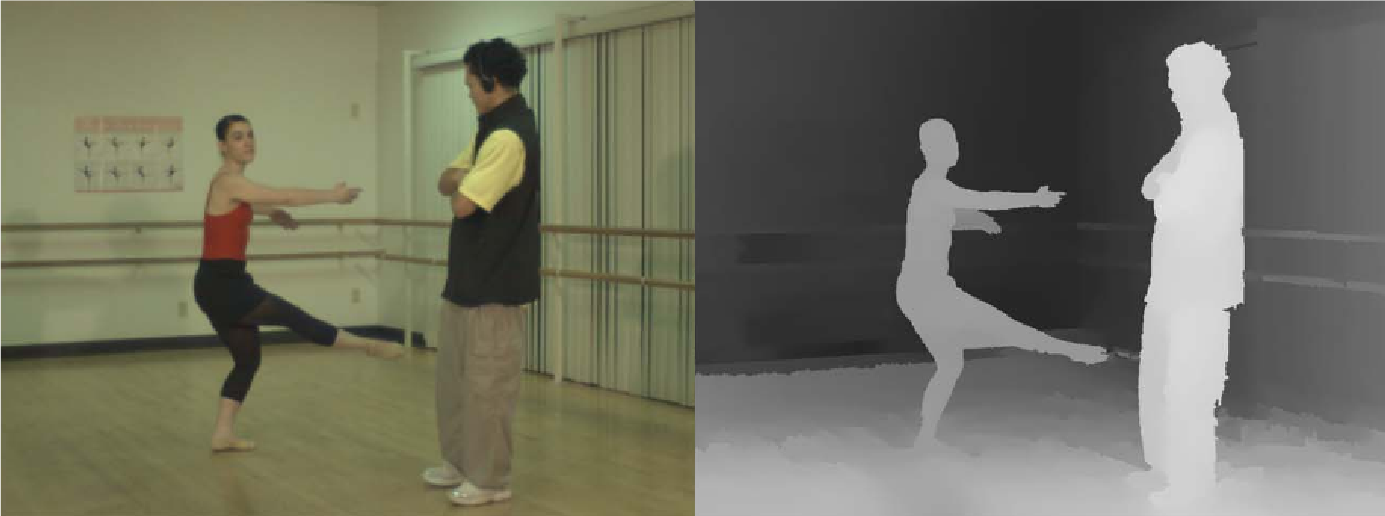
\includegraphics[width=0.66\textwidth]{images/depth_map.png}
	\caption{Depth Map eines 2D-Farbbilds. Entnommen aus \cite[S.649]{muller2010depth}}
	\label{fig:depth_map}
\end{figure}

Tiefenbilder haben im Vergleich zu anderen möglichen Datenmodellen den Vorteil, dass 2D-Bilder sehr einfach um zugehörige Tiefeninformationen erweitert werden können.
Jedoch gibt es auch einige Nachteile, die nicht umgangen werden können:

\begin{itemize}
\item Die 3D-Daten sind ausschließlich aus der Kameraperspektive vorhanden.
Um Informationen aus einer anderen Perspektive zu erhalten, muss erst aufwändig umgerechnet werden.
\item Da (in den meisten Fällen) nur ein zweidimensionales Array für die Tiefeninformation angelegt wird, können nur die Entfernungen zu den der Kamera nächsten Objekte gespeichert werden.
Verdeckte, reflektierende oder durchsichtige Oberflächen können nicht gespeichert werden.
\item Das Array ist an die Auflösung der Kamera gebunden.
Insbesondere bei großer Entfernung zu Objekten werden diese aufgrund des Bildwinkels sehr schlecht abgetastet, was später zu Aliasing-Effekten führen kann.
\item Die Bittiefe der Werte im Array kann - je nach gewünschter Auflösung - zu niedrig sein, bzw. muss erhöht werden.
Eine typische Farbtiefe eines Grauwertbilds von 8 Bit repräsentiert beispielsweise nur $2^8 = 256$ Stufen - was schnell zu wenig wird.
Insbesondere bei hoher notwendiger Auflösung im nahen Bereich, aber gleichzeitig vorhandenen weit entfernten Objekten kann dies zum Problem werden.
\end{itemize}


\subsection{Voxel Grid}
\label{subsec:voxel-grid}

Bei einem als Bitmap vorliegendes 2D-Bild werden die Bilddaten diskretisiert in einem zweidimensionalen Array $I$ gespeichert.
Mit einer Bittiefe $b$, einer Bildhöhe $i$ und einer Bildbreite $j$ ergibt sich damit folgende Matrix:

$$I = \begin{pmatrix}
v_{11} & v_{12} & v_{13} & \cdots\\
v_{21} & v_{22} & v_{23} & \cdots\\
v_{31} & v_{32} & v_{33} & \cdots\\
\vdots & \vdots & \vdots & \ddots
\end{pmatrix}, v_{ij} \in [0; 2^b) \wedge b, i, j \in \mathbb{N}^+$$

Dieses Prinzip lässt sich einfach auf den dreidimensionalen Raum erweitern.
Die so erhaltene Datenstruktur nennt sich Voxel Grid.
Als Voxel bezeichnet man somit eine einzelne Datenzelle im 3D-Array, also das dreidimensionale Äquivalent zum Pixel.

Voxel Grids finden in vielen Bereichen Anwendung, zum Beispiel in der Medizin \cite{van2008hippocampus, klein2009elastix, mohanty2012secure, roche1999towards} oder Geographie \cite{chmielewski2017estimating}.
Auch zum Downsampling von Punktwolken werden sie verwendet \cite{pclVoxelGrid}. %TODO Zu Punktwolken / Implementierung...

Gegenüber einem Tiefenbild hat ein Voxel Grid den inhärenten Nachteil, dass Speicherplatz für jeden Voxel benötigt wird.
Dies führt schnell zu großem Speicherbedarf $M$, da dieser kubisch zur Auflösung $r$ steigt: $M = r_x * r_y * r_z * b$ bei Bittiefe $b$.
Da der Speicher bereits bei der Initialisierung reserviert werden muss, ist die Änderung der Auflösung oder der Größe des abgedeckten Raumes unmöglich.
In diesem Fall müssen ein neues Voxel Grid (mit der neuen Auflösung bzw. Größe) angelegt und sämtliche Daten kopiert werden.

Zur Reduzierung des großen Speicherbedarfs werden deswegen häufig Baumstrukturen (sogenannte Octrees) eingesetzt.
Dabei wird der Raum in 8 Voxel geteilt, welche jeweils ein Blatt des Baumes darstellen.
Ist der Voxel gefüllt, wird er wieder entsprechend in 8 Untervoxel geteilt.
Dies wird wiederholt, bis die gewünschte Auflösung erreicht oder eine bestimmte Tiefe im Baum erreicht ist.
Szenen, die große Unterschiede in der Auflösung aufweisen oder viele leere Voxel beinhalten, brauchen so deutlich weniger Speicherplatz.

Ein Vorteil im Vergleich zum Tiefenbild ist jedoch, dass die Abhängigkeit von der Kameraperspektive wegfällt.
Dadurch können hier auch Objekte modelliert werden, die im Tiefenbild durch eine Verdeckung versteckt wären.
Desweiteren ist der Raum einheitlich diskretisiert.
Dies kann je nach Szene und Kameraposition sowohl ein Vor- als auch ein Nachteil sein:
Bei einem Tiefenbild nimmt der Abstand der Messpunkte mit der Tiefe ab.
Ist die Entfernung zwischen Objekt und Kamera gering, werden diese mit einer deutlich besseren Auflösung abgetastet als sehr weit entfernte Objekte.
Im Voxel Grid werden Objekte jedoch überall gleich abgetastet.
Dies führt zu verbesserter Auflösung bei entfernten und zu schlechterer Auflösung bei nahen Objekten.


\subsection{Punktwolken}
\label{subsec:punktwolken}

Ein weiteres häufig verwendetes Datenmodell ist eine Punktwolke.
Als Punktwolke bezeichnet man eine Menge $M \subset \mathbb{R}^3$ von Punkten im (mindestens) dreidimensionalen Raum.
Zusätzlich zur räumlichen Information können auch noch weitere Daten pro Punkt gespeichert sein, wie RGB-Werte, Genauigkeit oder Objektklasse (falls schon eine Segmentierung vorgenommen wurde).
Dadurch gilt:
$$M = \begin{pmatrix}
p_x^1 & p_y^1 & p_z^1 & \cdots\\
p_x^2 & p_y^2 & p_z^2 & \cdots\\
p_x^3 & p_y^3 & p_z^3 & \cdots\\
\vdots & \vdots & \vdots & \ddots
\end{pmatrix}$$

\begin{figure}[ht]
	\centering
	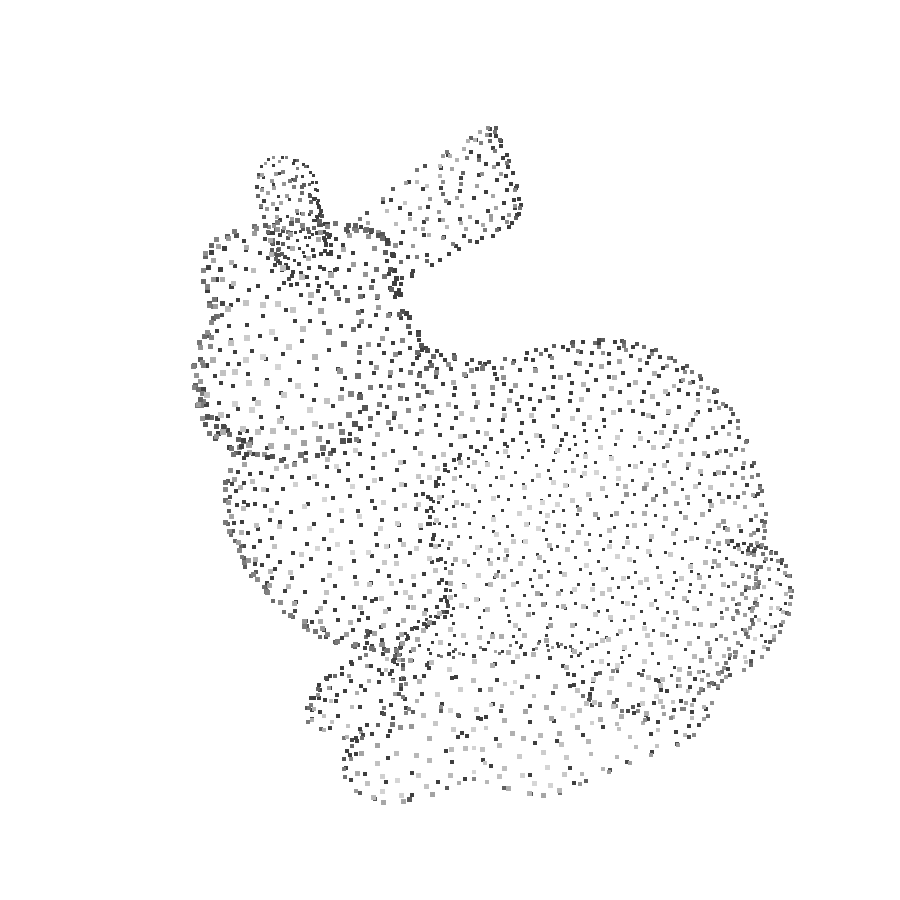
\includegraphics[width=0.66\textwidth, frame]{images/bunny_pcd.png}
	\caption{Punktwolke des Stanford Bunny \cite{stanfordbunny}}
	\label{fig:bunny_pcd}
\end{figure}

Die Nutzung von Punktwolken bringt im Vergleich zu anderen 3D-Datenmodellen einige Vorteile.

\begin{itemize}
\item Die zugrundeliegende Datenstruktur ist extrem trivial; es handelt sich um eine einfache Liste.
Dies ermöglicht sehr schnelle Operationen, wie zum Beispiel das Hinzufügen eines Punktes.
Es lässt sich sehr einfach über die Punkte iterieren.
\item Der Speicherbedarf einer Punktwolke wächst dynamisch, und zwar linear mit der Zahl der enthaltenen Punkte.
Beim Voxel Grid muss dagegen bereits am Anfang Speicher für jede Zelle reserviert werden, egal ob ein Punkt enthalten ist oder nicht.
\item Man ist nicht, wie beim Tiefenbild oder Voxelgrid, auf eine feste Anzahl an Punkten limitiert.
Beim Tiefenbild können maximal $n * m$ Punkte (ein Wert pro Pixel) mit einer Tiefeninformation versehen werden, beim Voxel Grid maximal $x * y * z$ Punkte (ein Wert pro Voxel).
Eine Kapazitätserweiterung, wie beispielsweise das Hinzufügen neuer Pixelspalten oder -zeilen im Tiefenbild, ist bei der Punktwolke nicht notwendig.
\item Die Auflösung ist nur durch die Gleitkommagenauigkeit der Maschine limitiert.
Beim Voxel Grid ist sie im Gegensatz dazu durch die Größe der Voxel limitiert.
Beim Tiefenbild ist die Auflösung abhängig von der Bittiefe und der z-Tiefe im Bild - bei weiter entfernten Objekten ist die Auflösung auch niedriger.
\end{itemize}

Es gibt jedoch auch einige Nachteile gegenüber den anderen Repräsentationen:

\begin{itemize}
\item Die Rekonstruktion eines Meshs ist nicht eindeutig.
Beim Voxel Grid lässt sich, beispielsweise mithilfe des Marching-Cubes-Algorithmus \cite{lorensen1987marching}, ein eindeutiges Mesh rekonstruieren.
Bei einer Punktwolke ist im Gegensatz dazu nicht festgelegt, welche Punkte miteinander verbunden werden sollen.
\item Viele bekannte Techniken aus der 2D-Bildverarbeitung (wie zum Beispiel Segmentierung, Filterung usw.) lassen sich auf Tiefenbilder direkt übertragen.
Dies ist bei Punktwolken nicht möglich.
\end{itemize}


\section{Meshrepräsentationen}
\label{sec:meshrepr}

Die bisher angesprochenen Datenstrukturen beinhalten ausschließlich Informationen über Punkte im dreidimensionalen Raum (Geometrie), nicht jedoch aber über die Relation, in der diese zueinander stehen (Topologie).
Das Polygonmesh erweitert diese Daten durch Kanteninformationen: Punkte (sogenannte Vertices) sind durch Kanten (Edges) miteinander verbunden.
Die so entstehenden Flächen der Polygone werden als Faces bezeichnet.
Da jedes Polygon in Dreiecke zerlegt werden kann, werden meist nur diese gespeichert.

\begin{figure}[ht]
	\centering
	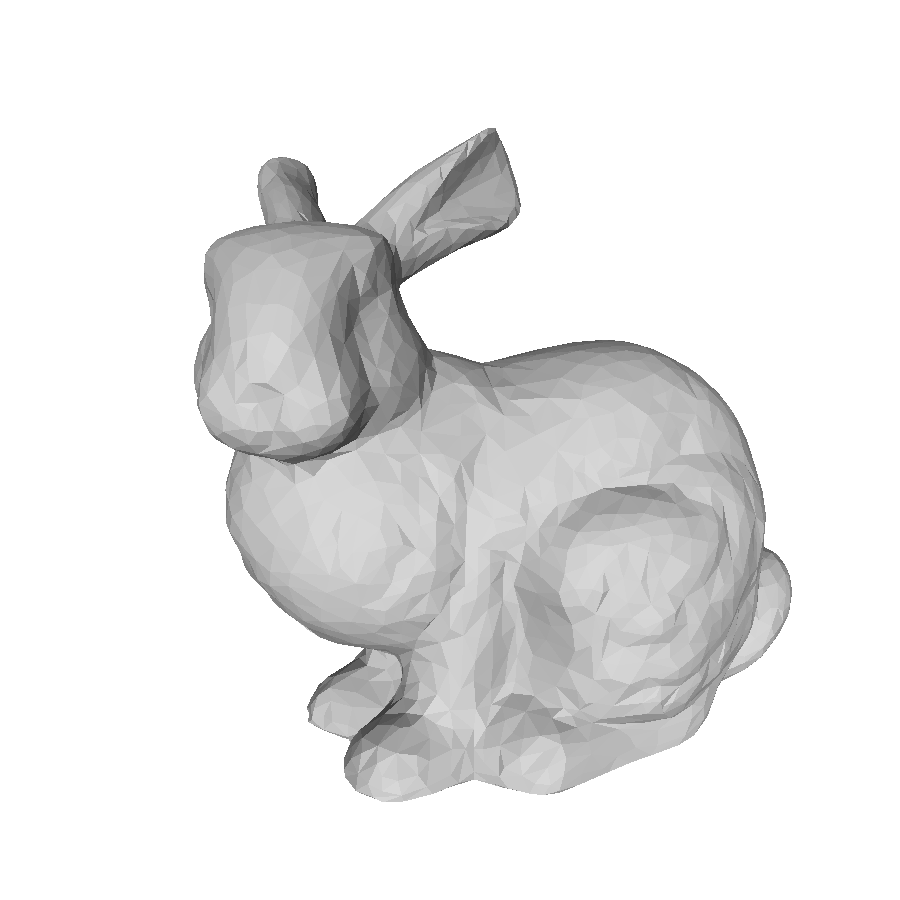
\includegraphics[width=0.66\textwidth, frame]{images/bunny_mesh.png}
	\caption{Mesh des Stanford Bunny \cite{stanfordbunny}}
	\label{fig:bunny_mesh}
\end{figure}

Vertices, Edges und Faces können in verschiedenen Repräsentationen gespeichert werden.
Diese haben unterschiedliche Eigenschaften und Vor- und Nachteile, die im folgenden genauer beleuchtet werden.

\subsection{\acl{VVM}}
\label{subsec:v-v-mesh}

Beim \ac{VVM} werden nur Vertices gespeichert, Kanten und Flächen ergeben sich implizit.
Existiert beispielsweise eine Verbindung zwischen den Vertices $v_1$ und $v_2$, $v_2$ und $v_3$ sowie $v_3$ und $v_1$ (ein einfaches Dreieck), werden die Werte in \autoref{tab:vvm-vertex-table} in einer Liste gespeichert:

\begin{table}[ht]
\centering
\begin{tabular}{| l | l |}
	\hline
	Vertex & verbundene Vertices\\
	\hline
	$v_1$ & $v_2, v_3$\\
	$v_2$ & $v_1, v_3$\\
	$v_3$ & $v_1, v_2$\\
	\hline
\end{tabular}
\caption{Vertextabelle beim \ac{VVM}}
\label{tab:vvm-vertex-table}
\end{table}

Der Speicherbedarf dieser simplen Darstellung ist sehr gering.
Die Einträge in der Tabelle können als Indizes der Vertexliste gespeichert werden.
Weiterhin sind Vertex-basierte Operationen sehr schnell.
Zum Hinzufügen eines Knotens muss beispielsweise nur ein neuer Eintrag in der Liste angelegt werden, sowie der neue Knoten zu den verbundenen Vertices hinzugefügt werden.

Um jedoch Informationen zu bestimmten Kanten oder Flächen zu bekommen, muss über die gesamte Liste iteriert werden.
Dies ist sehr langsam und schränkt den praktischen Nutzen von \acp{VVM} stark ein.

Ein Vergleich und eine Abwägung der Vor- und Nachteile mit anderen Datenstrukturen findet sich in \cite[Kap. 11]{smith2006vertex}.
Neben dem \ac{VVM} kann man in beliebigen Kombinationen auch Listen für Kanten oder Faces hinzufügen.
Dies erhöht zwar den Speicherbedarf und die Komplexität der Datenstruktur, bestimmte Zugriffe werden dadurch jedoch stark beschleunigt.


\subsection{Winged Edge}
\label{subsec:winged-edge}

In der Winged-Edge-Datenstruktur \cite{baumgart1975polyhedron} werden sowohl Vertices als auch Edges und Faces explizit abgespeichert.
Diese Repräsentation ermöglicht es, die Geometrie des Meshes im Vergleich zu anderen Strukturen leichter zu verändern.
Der Nachteil ist jedoch, dass der Speicheraufwand sehr hoch und die Datenstruktur im Vergleich zu den anderen Darstellungen sehr komplex ist.

Bei der Winged-Edge-Darstellung werden in der Kantentabelle jeweils die vorhergehenden und nachfolgenden Kanten im und gegen den Uhrzeigersinn gespeichert. Dies ermöglicht die schnelle Bestimmung von angrenzenden Kanten, Vertices oder Faces, bedeutet aber gleichzeitig auch viel Verwaltungsaufwand der Indizes. In \autoref{fig:winged-edge-edges} findet sich eine Übersicht über die entsprechenden Kanten.

\begin{figure}[ht]
\centering
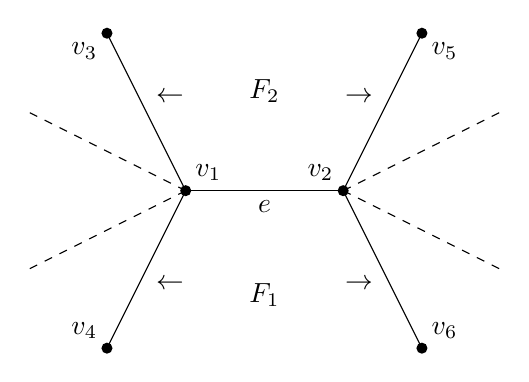
\begin{tikzpicture}[scale=2]
\coordinate[label=45:$v_1$] (v_1) at (1,1);
\coordinate[label=135:$v_2$] (v_2) at (2,1);
\coordinate[label=-135:$v_3$] (v_3) at (0.5,2);
\coordinate[label=135:$v_4$] (v_4) at (0.5,0);
\coordinate[label=-45:$v_5$] (v_5) at (2.5,2);
\coordinate[label=45:$v_6$] (v_6) at (2.5,0);
\coordinate[label=$F_1$] (F_1) at (1.5,0.2);
\coordinate[label=$F_2$] (F_2) at (1.5,1.5);
\draw (v_1) to node[below]{$e$} (v_2);
\draw (v_1) to node[above right]{$\leftarrow\circlearrowleft$} (v_3);
\draw (v_1) to node[below right]{$\leftarrow\circlearrowright$} (v_4);
\draw (v_2) to node[above left]{$\rightarrow\circlearrowleft$} (v_5);
\draw (v_2) to node[below left]{$\rightarrow\circlearrowright$} (v_6);
\draw[dashed] (v_1) to (0,1.5);
\draw[dashed] (v_1) to (0,0.5);
\draw[dashed] (v_2) to (3,1.5);
\draw[dashed] (v_2) to (3,0.5);
\fill (v_1) circle (1pt);
\fill (v_2) circle (1pt);
\fill (v_3) circle (1pt);
\fill (v_4) circle (1pt);
\fill (v_5) circle (1pt);
\fill (v_6) circle (1pt);
\end{tikzpicture}
\caption{Vor- und Nachfolgerkanten der Winged-Edge-Datenstruktur (nach \cite[S.591]{baumgart1975polyhedron})}
\label{fig:winged-edge-edges}
\end{figure}

Die in \autoref{fig:winged-edge-triangles} gezeigte Darstellung von zwei beispielhaften Dreiecken $(v_1, v_2, v_3)$ und $(v_2, v_4, v_3)$ ist in \autoref{tab:winged-edge-table} dargestellt.

\begin{figure}[ht]
\centering
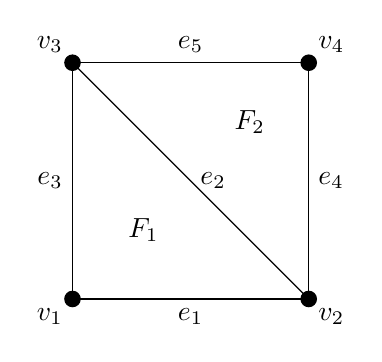
\begin{tikzpicture}[scale=3]
\coordinate[label=-135:$v_1$] (v_1) at (0,0);
\coordinate[label=-45:$v_2$] (v_2) at (1,0);
\coordinate[label=135:$v_3$] (v_3) at (0,1);
\coordinate[label=45:$v_4$] (v_4) at (1,1);
\coordinate[label=$F_1$] (F_1) at (0.3,0.2);
\coordinate[label=$F_2$] (F_2) at (0.75,0.66);
\draw (v_1) to node[below]{$e_1$} (v_2);
\draw (v_2) to node[right]{$e_2$} (v_3);
\draw (v_3) to node[left]{$e_3$} (v_1);
\draw (v_2) to node[right]{$e_4$} (v_4);
\draw (v_4) to node[above]{$e_5$} (v_3);
\fill (v_1) circle (1pt);
\fill (v_2) circle (1pt);
\fill (v_3) circle (1pt);
\fill (v_4) circle (1pt);
\end{tikzpicture}
\caption{Beispieldreiecke zur Winged-Edge-Datenstruktur}
\label{fig:winged-edge-triangles}
\end{figure}

\begin{table}[ht]
\centering
% Edges
\begin{tabular}{| l | l | l | l | l | l | l |}
\hline
\multicolumn{7}{| c |}{\textbf{Edges}}\\
\hline\hline
Edge & Vertices & Faces & $\leftarrow \circlearrowleft$ & $\leftarrow \circlearrowright$ & $\rightarrow \circlearrowleft$ & $\rightarrow \circlearrowright$\\
\hline
$e_1$ & $v_1, v_2$ & $F_1$ & $e_3$ & $e_3$ & $e_2$ & $e_4$\\
$e_2$ & $v_2, v_3$ & $F_1, F_2$ & $e_1$ & $e_4$ & $e_3$ & $e_5$\\
$e_3$ & $v_3, v_1$ & $F_1$ & $e_2$ & $e_5$ & $e_1$ & $e_1$\\
$e_4$ & $v_2, v_4$ & $F_2$ & $e_2$ & $e_1$ & $e_5$ & $e_5$\\
$e_5$ & $v_4, v_3$ & $F_2$ & $e_4$ & $e_4$ & $e_2$ & $e_3$\\
\hline
\multicolumn{7}{}{}\\
\cline{1-2}\cline{6-7}
\multicolumn{2}{| c |}{\textbf{Vertices}} & \multicolumn{3}{}{} & \multicolumn{2}{| c |}{\textbf{Faces}}\\
\cline{1-2}\cline{6-7}\noalign{\vskip\doublerulesep\vskip-\arrayrulewidth}\cline{1-2}\cline{6-7}
Vertex & Edges & \multicolumn{3}{c|}{} & Face & Edges\\\cline{1-2}\cline{6-7}
$v_1$ & $e_1, e_3$ & \multicolumn{3}{c|}{} & $F_1$ & $e_1, e_2, e_3$\\
$v_2$ & $e_1, e_2, e_4$ & \multicolumn{3}{c|}{} & $F_2$ & $e_4, e_5, e_2$\\\cline{6-7}
$v_3$ & $e_2, e_3, e_5$ & \multicolumn{5}{}{}\\
$v_4$ & $e_4, e_5$ & \multicolumn{5}{}{}\\\cline{1-2}
\end{tabular}
\caption{Vertex-, Edge- und Face-Tabellen zu \autoref{fig:winged-edge-triangles}}
\label{tab:winged-edge-table}
\end{table}


%TODO Half-edge
\subsection{Half Edge}
\label{subsec:half-edge}


\section{Point Cloud Library}
\label{sec:pcl}

Bei der \ac{PCL} \cite{rusu2011pcl} handelt es sich um eine Bibliothek, welche die Arbeit mit 3D-Punktwolken immens vereinfacht.
Sie bietet Möglichkeiten zur Filterung, Segmentierung, Oberflächenrekonstruktion und Visualisierung von Punktwolken, sowie weitere Module.

Neben den zahlreichen unterstützten Anwendungsgebieten und implementierten Algorithmen bietet die \ac{PCL} den weiteren entscheidenden Vorteil, dass sie direkt zu \ac{ROS} kompatibel ist.
Die Kompatibilität wird durch ROS-Nodelets im Paket \texttt{perception\_pcl} hergestellt, sodass Punktwolken, Meshes oder andere Datenstrukturen direkt per Message versendet werden können.
